% Options for packages loaded elsewhere
\PassOptionsToPackage{unicode}{hyperref}
\PassOptionsToPackage{hyphens}{url}
\PassOptionsToPackage{dvipsnames,svgnames,x11names}{xcolor}
%
\documentclass[
  letterpaper,
  DIV=11,
  numbers=noendperiod]{scrreprt}

\usepackage{amsmath,amssymb}
\usepackage{iftex}
\ifPDFTeX
  \usepackage[T1]{fontenc}
  \usepackage[utf8]{inputenc}
  \usepackage{textcomp} % provide euro and other symbols
\else % if luatex or xetex
  \usepackage{unicode-math}
  \defaultfontfeatures{Scale=MatchLowercase}
  \defaultfontfeatures[\rmfamily]{Ligatures=TeX,Scale=1}
\fi
\usepackage{lmodern}
\ifPDFTeX\else  
    % xetex/luatex font selection
\fi
% Use upquote if available, for straight quotes in verbatim environments
\IfFileExists{upquote.sty}{\usepackage{upquote}}{}
\IfFileExists{microtype.sty}{% use microtype if available
  \usepackage[]{microtype}
  \UseMicrotypeSet[protrusion]{basicmath} % disable protrusion for tt fonts
}{}
\makeatletter
\@ifundefined{KOMAClassName}{% if non-KOMA class
  \IfFileExists{parskip.sty}{%
    \usepackage{parskip}
  }{% else
    \setlength{\parindent}{0pt}
    \setlength{\parskip}{6pt plus 2pt minus 1pt}}
}{% if KOMA class
  \KOMAoptions{parskip=half}}
\makeatother
\usepackage{xcolor}
\setlength{\emergencystretch}{3em} % prevent overfull lines
\setcounter{secnumdepth}{5}
% Make \paragraph and \subparagraph free-standing
\makeatletter
\ifx\paragraph\undefined\else
  \let\oldparagraph\paragraph
  \renewcommand{\paragraph}{
    \@ifstar
      \xxxParagraphStar
      \xxxParagraphNoStar
  }
  \newcommand{\xxxParagraphStar}[1]{\oldparagraph*{#1}\mbox{}}
  \newcommand{\xxxParagraphNoStar}[1]{\oldparagraph{#1}\mbox{}}
\fi
\ifx\subparagraph\undefined\else
  \let\oldsubparagraph\subparagraph
  \renewcommand{\subparagraph}{
    \@ifstar
      \xxxSubParagraphStar
      \xxxSubParagraphNoStar
  }
  \newcommand{\xxxSubParagraphStar}[1]{\oldsubparagraph*{#1}\mbox{}}
  \newcommand{\xxxSubParagraphNoStar}[1]{\oldsubparagraph{#1}\mbox{}}
\fi
\makeatother


\providecommand{\tightlist}{%
  \setlength{\itemsep}{0pt}\setlength{\parskip}{0pt}}\usepackage{longtable,booktabs,array}
\usepackage{calc} % for calculating minipage widths
% Correct order of tables after \paragraph or \subparagraph
\usepackage{etoolbox}
\makeatletter
\patchcmd\longtable{\par}{\if@noskipsec\mbox{}\fi\par}{}{}
\makeatother
% Allow footnotes in longtable head/foot
\IfFileExists{footnotehyper.sty}{\usepackage{footnotehyper}}{\usepackage{footnote}}
\makesavenoteenv{longtable}
\usepackage{graphicx}
\makeatletter
\def\maxwidth{\ifdim\Gin@nat@width>\linewidth\linewidth\else\Gin@nat@width\fi}
\def\maxheight{\ifdim\Gin@nat@height>\textheight\textheight\else\Gin@nat@height\fi}
\makeatother
% Scale images if necessary, so that they will not overflow the page
% margins by default, and it is still possible to overwrite the defaults
% using explicit options in \includegraphics[width, height, ...]{}
\setkeys{Gin}{width=\maxwidth,height=\maxheight,keepaspectratio}
% Set default figure placement to htbp
\makeatletter
\def\fps@figure{htbp}
\makeatother

\KOMAoption{captions}{tableheading}
\makeatletter
\@ifpackageloaded{bookmark}{}{\usepackage{bookmark}}
\makeatother
\makeatletter
\@ifpackageloaded{caption}{}{\usepackage{caption}}
\AtBeginDocument{%
\ifdefined\contentsname
  \renewcommand*\contentsname{Tabla de contenidos}
\else
  \newcommand\contentsname{Tabla de contenidos}
\fi
\ifdefined\listfigurename
  \renewcommand*\listfigurename{Listado de Figuras}
\else
  \newcommand\listfigurename{Listado de Figuras}
\fi
\ifdefined\listtablename
  \renewcommand*\listtablename{Listado de Tablas}
\else
  \newcommand\listtablename{Listado de Tablas}
\fi
\ifdefined\figurename
  \renewcommand*\figurename{Figura}
\else
  \newcommand\figurename{Figura}
\fi
\ifdefined\tablename
  \renewcommand*\tablename{Tabla}
\else
  \newcommand\tablename{Tabla}
\fi
}
\@ifpackageloaded{float}{}{\usepackage{float}}
\floatstyle{ruled}
\@ifundefined{c@chapter}{\newfloat{codelisting}{h}{lop}}{\newfloat{codelisting}{h}{lop}[chapter]}
\floatname{codelisting}{Listado}
\newcommand*\listoflistings{\listof{codelisting}{Listado de Listados}}
\makeatother
\makeatletter
\makeatother
\makeatletter
\@ifpackageloaded{caption}{}{\usepackage{caption}}
\@ifpackageloaded{subcaption}{}{\usepackage{subcaption}}
\makeatother

\ifLuaTeX
\usepackage[bidi=basic]{babel}
\else
\usepackage[bidi=default]{babel}
\fi
\babelprovide[main,import]{spanish}
% get rid of language-specific shorthands (see #6817):
\let\LanguageShortHands\languageshorthands
\def\languageshorthands#1{}
\ifLuaTeX
  \usepackage{selnolig}  % disable illegal ligatures
\fi
\usepackage{bookmark}

\IfFileExists{xurl.sty}{\usepackage{xurl}}{} % add URL line breaks if available
\urlstyle{same} % disable monospaced font for URLs
\hypersetup{
  pdftitle={Bitácoras Grupo \#2, CA-204 (II-2024)},
  pdfauthor={Gabriel Sanabria Alvarado, Paola Espinoza Hernández},
  pdflang={es},
  colorlinks=true,
  linkcolor={blue},
  filecolor={Maroon},
  citecolor={Blue},
  urlcolor={Blue},
  pdfcreator={LaTeX via pandoc}}


\title{Bitácoras Grupo \#2, CA-204 (II-2024)}
\author{Gabriel Sanabria Alvarado, Paola Espinoza Hernández}
\date{2024-09-05}

\begin{document}
\maketitle

\renewcommand*\contentsname{Tabla de contenidos}
{
\hypersetup{linkcolor=}
\setcounter{tocdepth}{2}
\tableofcontents
}

\bookmarksetup{startatroot}

\chapter*{Introducción}\label{introducciuxf3n}
\addcontentsline{toc}{chapter}{Introducción}

\markboth{Introducción}{Introducción}

El presente trabajo busca realizar un análisis de una base de datos con
el fin de decifrar las tendencia globales en energía renovable y
examinar el progreso de diversos indicadores a través de los años

\bookmarksetup{startatroot}

\chapter{Energía del Futuro: Análisis Global de Tendencias e Indicadores
en Energías
Renovables}\label{energuxeda-del-futuro-anuxe1lisis-global-de-tendencias-e-indicadores-en-energuxedas-renovables}

\bookmarksetup{startatroot}

\chapter{Bitácora 1}\label{bituxe1cora-1}

\section{Changelog}\label{changelog}

\begin{center}
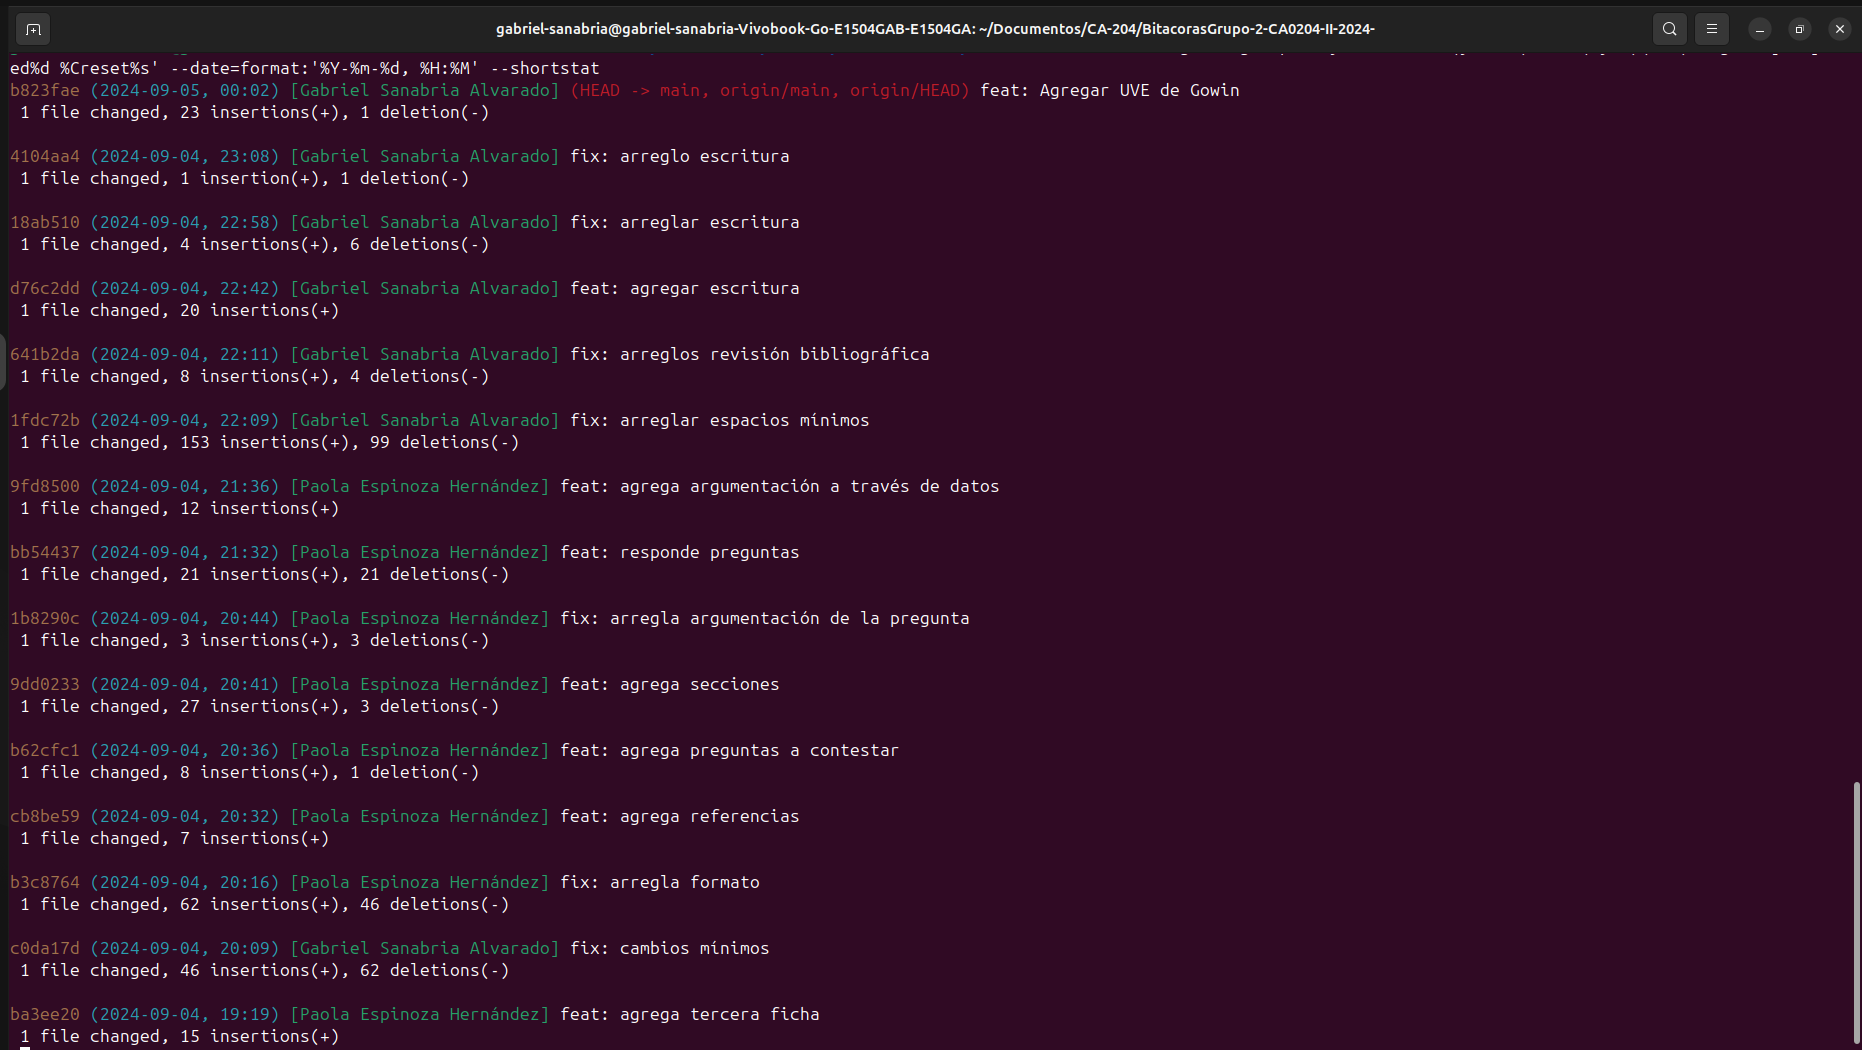
\includegraphics[width=0.8\textwidth,height=\textheight]{capturagitlog.png}
\end{center}

\begin{figure}[H]

{\centering 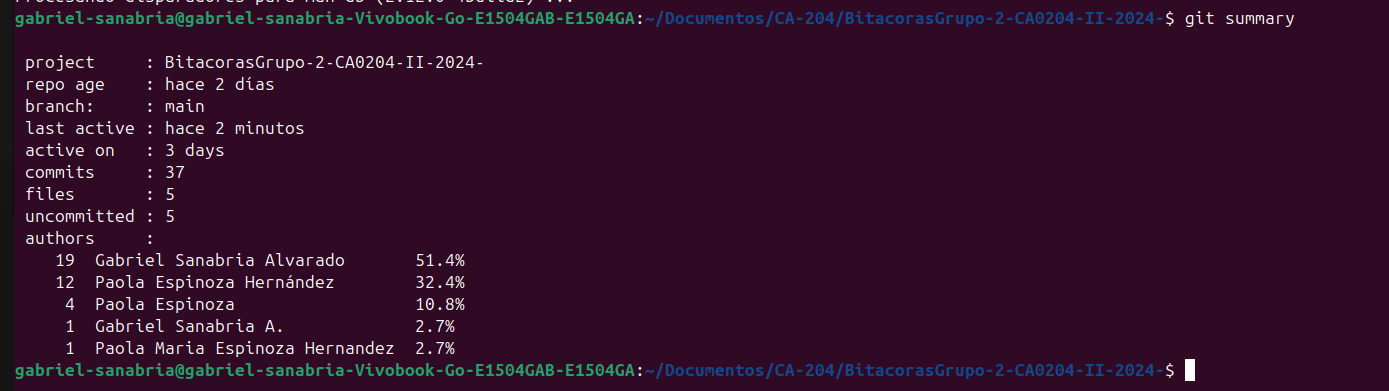
\includegraphics[width=0.8\textwidth,height=\textheight]{git-summary.png}

}

\caption{Git summary}

\end{figure}%

\section{Planificación}\label{planificaciuxf3n}

\subsection{Pregunta de
Investigación}\label{pregunta-de-investigaciuxf3n}

¿Qué impacto puede tener la energía renovable sobre la sociedad?

Definición de la idea La idea inicial consiste en abordar la energía
renovable, su producción, utilización, el intercambio que se da entre
países; así como el impacto que la utilización de energías renovables
puede tener sobre la sociedad como conjunto. Este tema resulta
interesante, especialmente bajo el contexto actual, puesto que es usual
pensar en las energías renovables para combatir el cambio climático; sin
embargo, no es tan común escuchar del impacto social que esta produce,
ejemplo de ello es el cambio en los paisajes que señala Requejo en el
2012, la posibilidad de alterar el abastecimiento energético que señalan
Casola y Freier en el 2018, o los efectos económicos que plantean
Caraballo y García en el 2017. Este trabajo pretende abordar no solo la
parte de la energía como tal, sino su impacto en los países que la
produce y utilizan. De esta manera, la idea se resume en: Considerar la
producción de energías renovales en diversos países, y el impacto que
esto tiene sobre ellos.

\subsection{Conceptualización de la idea Según la RAE, las definiciones
de las palabras utilizadas en la idea
son:}\label{conceptualizaciuxf3n-de-la-idea-seguxfan-la-rae-las-definiciones-de-las-palabras-utilizadas-en-la-idea-son}

\textbf{Considerar:} Pensar, meditar, reflexionar algo con atención y
cuidado.

\textbf{Impacto:} Huella o señal que deja.

\textbf{Energía renovable:} Energía que procede de un recurso presente
en la naturaleza de manera prácticamente inagotable.

\textbf{Prácticamente:} Casi, por poco.

\subsection{Identificación de tensiones Las comparaciones entre países
puede verse afectadas por el contexto del país, importación y
exportación de energía, los recursos naturales y el tipo de energía
renovable producida en cada
país.}\label{identificaciuxf3n-de-tensiones-las-comparaciones-entre-pauxedses-puede-verse-afectadas-por-el-contexto-del-pauxeds-importaciuxf3n-y-exportaciuxf3n-de-energuxeda-los-recursos-naturales-y-el-tipo-de-energuxeda-renovable-producida-en-cada-pauxeds.}

\subsection{Reformulación de la idea en modo de
pregunta}\label{reformulaciuxf3n-de-la-idea-en-modo-de-pregunta}

\textbf{¿Qué impacto puede tener la energía renovable sobre la
sociedad?}

\textbf{¿Cómo puedo comparar los países en materia de enegías
renovables?}

\textbf{¿Puede la utilización de energías renovables garantizar un
futuro sostenible?}

\textbf{¿Cuáles factores afectan la producción de energía renovable?}

\subsubsection{Argumentación de la
pregunta}\label{argumentaciuxf3n-de-la-pregunta}

\textbf{Pregunta: ¿Qué impacto puede tener la energía renovable sobre la
sociedad?}

\textbf{Contraargumentos}

-\textbf{Ética:} La inversión de energía renovable podría llegar a ser
costosa, por lo que podrían salir perjudicados lo grupos más
vulnerables.

-\textbf{Lógica:} Las energías renovables como lo son la energía solar y
eólica pueden no estar disponible dependiendo de la zona donde estén
instaladas.

-\textbf{Emocional:} La implementación de energías renovables podrían
ser perjudiciales en tema de pérdida de empleo en compañías de
electricidad tradicionales.

\textbf{Argumentos}

-\textbf{Lógica:}La energía producida con fuentes no renovables implica
un riego a su propia sostenibilidad, además de la enorme contaminación
que genera.

-\textbf{Ética:} A pesar de que la inversión de la instalación de
energías renovables podría ser costosa, a largo plazo, las pérdidas que
genería el hecho de no realizar la instalación son mayores en temas de
salud ambiental y pública. La presente generación está moralmente
obligada a un correcto manejo de los recursos naturales. El uso de
fuentes no renovables perjudica y acelera los distintos cambios
climáticos, los cuales pueden afectar gravemente a las futuras
generaciones.

-\textbf{Emocional:} El uso de energías renovables puede provocar un
mejoramiento en el estilo de vida de los próximos años en comparación a
las expectativas del presente. Ocasionando que futuras familias y
sociedades puedan tener un mejor desarrollo colectivo e individual.

-\textbf{Conclusión:} La importancia de las energías renovables van más
allá de combatir el cambio climático y la contaminación ambiental,
debido a que esto genera mejorías en el desarrollo socio-económico,
además de un aumento en la salud pública internacional.

\textbf{Pregunta: ¿Cuáles factores afectan la producción de energía
renovable?}

\textbf{Contrargumentos}

-\textbf{Lógica:} Hay un gran número de factores que afectan dicha
producción, algunos difíciles de conseguir. No es posible contabilizar
cada uno de estos factores, pues algunos, como la estacionalidad son
variables.

-\textbf{Ética:} La distribución de las plantas generadoras de energía
genera una brecha entre la capacidad de producción energética entre
diversas poblaciones de una misma región.

-\textbf{Emocional:} La desinformación de los habitantes de una nación
puede desincentivar la transición hacia las energías renovables, pues no
habrán incentivos por parte de esta población a la inversión en
investigación y desarrollo de mecanismos para generar energía renovable.

\textbf{Argumentos}

-\textbf{Lógica:} Si bien existen muchos factores que inciden en el
nivel de producción de la energía, se pueden incluir varios de estos
factores, en particular los que resulten más relevantes, como la
temperatura promedio anual, cantidad de lluvia, irradiación solar,
incidencia de desastres naturales, velocidad del viento, disponibilidd
de biomasa, y potencial hídrico y geotérmico.

-\textbf{Ética:} Es posible recolectar datos que muestren la
concentración de estas plantas, ajustar las mediciones con respecto a
alguna otra variable, como la población o el nivel de industrialización.

-\textbf{Emocional:} Los programas de conscientización son una parte
importante en la transición a las energías renovables; por lo tanto,
esta puede ser tomada en cuenta para el análisis, así como la inversión
en investigación y desarrollo.

-\textbf{Conclusión:} En la comparación entre países, se deben
incorporar diversos factores que impacten a la producción de energía.
Dichos factores incluyen los recursos naturales, el avance tecnológico,
las políticas, las condiciones ambientales, la consciencia de la
población y la tasa de industrialización.

\textbf{Pregunta: ¿Cómo puedo comparar los países en materia de enegías
renovables?}

\textbf{Contrargumentos}

-\textbf{Lógica:} Para comparar los países, se deben tomar en cuenta las
diferencias entre países, más allá de los montos nominales.

-\textbf{Ética:} No todos los países cuentan con la misma capacidad de
inversión, ni el mismo nivel de vida. Comparar países sin incluir estos
factores no resultaría en una buena comparación.

-\textbf{Emocional:} Las energías renovables suelen pasar desapercibidas
ante los habitantes de las naciones, pues estos no se mantienen
informados sobre el nivel de autosuficiencia energética que posee su
país, ni la cantidad de energía exportada en lugar de utilizarse en el
mismo.

\textbf{Argumentos}

-\textbf{Lógica:} Se pueden incorporar diversas variables al análisis
con el fin de hacer una comparación más justa, incluyendo el GDP, del
cual se podrá sacar el porcentaje destinado a inversión en investigación
para la producción de energía renovable.

-\textbf{Ética:} Es posible incorporar variables sociales, que muestren
la calidad de vida de las personas, y realizar un análisis sobre el
impacto que la transición a la energía renovable representa en la vida
de los habitantes.

-\textbf{Emocional:} Los datos sobre exportación e importación de
energía son muy relevantes, espacialmente cuando se habla de
autosuficiencia. Del mismo modo, la conscientización de la población es
un factor que debe ser considerado en el análisis.

-\textbf{Conclusión:} Para comparar países en términos de energías
renovables, es importante evaluar varios aspectos clave. Se debe
considerar la energía generada y la consumida; la capacidad instalada,
así como la producción anual. Además, se deben analizar las inversiones
realizadas, los costos de instalación y mantenimiento, y las políticas
gubernamentales que fomenten el uso de energías renovables.

\textbf{Pregunta: ¿Puede la utilización de energías renovables
garantizar un futuro sostenible?}

\textbf{Contrargumentos}

-\textbf{Lógica:} Se necesitan más herramientas, especialmente a nivel
global, para lograr un futuro sostenible, pues la energía renovable por
sí misma, no es capaz de garantizar un futuro sostenible.

-\textbf{Ética:} El futuro sostenible no debería considerar únicamente
las energías renovables, sino velar por un mundo mejor, con menores
emisiones de gases de efecto invernadero, y un mayor desarrollo
económico.

-\textbf{Emocional:} La energía renovable no es capaz de solucionar el
problema; además, pone en peligro el abastecimiento energético de los
países en transición.

\textbf{Argumentos}

-\textbf{Lógica:} Si bien la energía renovable por sí misma no va a
garantizar un futuro sostenible, sí corresponde a una buena herramienta
en este proceso. Además, al utilizar energía renovable, se está dando el
primer paso hacia la meta del futuro sostenible.

-\textbf{Ética:} Es imperante en el contexto actual, analizar la
relación entre el desarrollo económico y la energía renovable.
Adicionalmente, la utilización de energía renovable puede representar el
inicio de un camino hacia un futuro mejor, pues reduce las emisiones de
CO2; también es necesario invertir en investigación para desarrollar
maneras de crear un menor impacto ambiental.

-\textbf{Emocional:} La inversión en el desarrollo y mejoramiento de la
producción de energías renovables puede solucionar muchos de los
problemas derivados de esto. Existe además el concepto de
autosuficiencia conectada, que puede ser de ayuda a los países en etapa
de transición.

-\textbf{Conclusión:} La utilización de energías renovables es
fundamental para un futuro sostenible al reducir emisiones de gases de
efecto invernadero, diversificar la matriz energética y fomentar el
desarrollo económico. Sin embargo, no garantiza la sostenibilidad por sí
misma; puesto que algunas tecnologías poseen un impacto ambiental, y se
necesita de políticas y regulaciones adecuadas. Así, las energías
renovables son vitales para un futuro sostenible, pero deben unirse a
otros esfuerzos.

\subsubsection{Argumentación a través de
datos}\label{argumentaciuxf3n-a-travuxe9s-de-datos}

\textbf{Fuente de información:} Es una compilación de diversos
indicadores sobre la energía renovable, incluyendo la producción,
inversión y capacidad, así como factores socio-económicos y ambientales.
Se encuentra disponible en kaggle.com,
https://www.kaggle.com/datasets/anishvijay/global-renewable-energy-and-indicators-dataset

\textbf{Contexto temporal y espacial de los datos:} Los datos comprenden
del 2000 al 2023, en los países de Australia, Brazil, Canadá, China,
Francia, Alemania, India, Japón, Rusia y Estados Unidos. Al respecto, se
destaca que los países destacan en cuanta al desarrollo. Por otro lado,
los datos son bastante recientes, lo que aumenta el nivel de
conscientización en el tema de la contaminación ambiental.

\textbf{Facilidad de obtener la información:} Compilación de datos, con
el fin de ayudar al estudio de tendencias, impactos y estrategias
relacionados a la implementación de la energía renovable. Población de
estudio: Australia, Brazil, Canadá, China, Francia, Alemania, India,
Japón, Rusia y Estados Unidos.

\textbf{Muestra observada:} Datos obtenidos sobre la población de
Australia, Brazil, Canadá, China, Francia, Alemania, India, Japón, Rusia
y Estados Unidos. Incluye indicadores sociales como la estabilidad
política, el nivel educativo, el índice de percepción de la corrupción.

\textbf{Unidad estadística:} Australia, Brazil, Canadá, China, Francia,
Alemania, India, Japón, Rusia y Estados Unidos.

\textbf{Descripción de variables de la tabla:} Se incluyen los países y
los años, para realizar comparaciones no solo consigo mismos sino entre
ellos. Los tipos de energía incluyen la solar, geotérmica, biomasa,
eólica e hidroeléctrica; esos datos se utilizaran junto con la
producción, la emisión de CO2, y la capacidad instalada, para tener una
mejor comprensión acerca de la capacidad productiva, y realizar mejores
comparaciones, entrelazando estos datos con la existencia de alianzas
publico-privadas y de cooperación regional. Se realizaran análisis sobre
la inversión, en búsqueda del impacto que esta pueda tener sobre las
demás variables. La población se utilizará para comparar el GDP (Gross
Domestic Product) y el consumo energético; el GDP es el valor final de
todos los bienes y servicios producidos dentro de un país. La
importación y exportación de energía se utilizará para analizar el nivel
de autosuficiencia de los países. Aunado a ello, se enfatizará en la
proporción de la energía que procede de fuentes renovables. Con respecto
a la utilización de los recursos, se utilizarán los datos de temperatura
promedio anual, cantidad de lluvia, irradiación solar, velocidad del
viento, disponibilidd de biomasa, y potencial hídrico y geotérmico; así
como la incidencia de desastres naturales en el año. De igual manera, se
tomarán en cuenta la capacidad de almacenaje, si el mercado está o no
liberalizado, la cantidad de patentes para energía renovable y la ayuda
internacional para energía renovable. Para el análisis del impacto
social, se consideran los precios de la electricidad, subsidios a
energía, la consciencia de la población, la tasa de urbanización e
industrialización, el nivel educativo, la existencia de programas de
educación sobre la energía renovable, el índice de percepción de la
corrupción y la calidad regulatoria (percepción de abilidad del gobierno
para formular e implementar regulaciones que permitan el desarrollo de
un sector). Se analizará el papel del gobierno en cuanto a si existen o
no políticas públicas y programas de eficiencia energética, objetivos
con respecto a la energía renovable, la existencia de acuerdos de
trnsferencia energética, las tarifas al equipo para energía, los
incentivos a la exportación de equipo, así como la inversión en
investigación y desarrollo (R\&D), el número de instituciones de
investigación, el índice de innovación, el número de conferencias sobre
energía y el número de publicaciones sobre dicha energía. Así mismo, se
compará la estabilidad política, el índice de libertad económica, y la
facilidad para hacer negocios. Por último, se buscarán tendencias en la
fuerza de trabajo dedicda al sector de energía renovable.

\section{Revisión Bibliográfica}\label{revisiuxf3n-bibliogruxe1fica}

Agencia Internacional de Energías Renovables (IRENA). (2021).
\emph{Renewable Energy Statistics 2021}.
https://www.irena.org/Statistics

Bataineh, M. J., Marcuello, C., \& Sánchez-Sellero, P. (2023). Toward
sustainability: the role of social entrepreneurship in creating
social-economic value in renewable energy social enterprises.
\emph{REVESCO : Revista De Estudios Cooperativos, 143}.
https://doi.org/10.5209/reve.85561

Casamitjana, M. (2017). Energías renovables. Revista Cintex, 22(1), 7-9.
https://proquest.proxyucr.elogim.com/scholarly-journals/energías-renovables/docview/2676149315/se-2

Cordero Gutiérrez, A. (2015). \emph{Análisis de viabilidad ambiental del
uso de energías renovables en Costa Rica: Estudio de caso de la energía
eólica, la hidroeléctrica y la geotérmica}.
https://d1wqtxts1xzle7.cloudfront.net/41694115/Investigacion\_p.\_Ecologicos2-libre.pdf

Esteves, A. M., Franks, D. M., \& Vanclay, F. (2012). Social impact
assessment: the state of the art. \emph{Impact Assessment and Project
Appraisal, 30}(1), 34-42. https://doi.org/10.1080/14615517.2012.660356

Holme, J., Pockrandt, M., Köhler, D., Noll, M., Zaytsev, Y., Attia, S.,
\& Biurrun, I. (2023). \emph{Effects of plant invaders on native
vegetation communities and ecosystem properties across Europe: A
systematic review and meta-analysis. PLOS ONE, 18}(8), e0299807.
https://doi.org/10.1371/journal.pone.0299807

Peake, S., \& Boyle, G. (2018). \emph{Renewable energy: Power for a
sustainable future (4th ed.)}. Oxford University Press.

Pou, M. Á. C., \& Simón, J. M. G. (2017). Energías renovables y
desarrollo económico. Un análisis para España y las grandes economías
europeas.
\[Renewable Energy and Economic Development. An Analysis for Spain and the Biggest European Economies\]
\emph{El Trimestre Económico, 84}(3), 571-609.
https://doi.org/10.20430/ete.v84i335.508

Requejo Liberal, J. (2012). Energía renovable: un nuevo principio de
autosuficiencia conectada. Ciudad Y Territorio Estudios Territoriales,
44(171), 113--125.
https://recyt.fecyt.es/index.php/CyTET/article/view/76112

Serrano, J. (2022, Apr 24). Hacia un futuro con energía limpia y
renovable. Actualidad Economica, , 12.
https://proquest.proxyucr.elogim.com/magazines/hacia-un-futuro-con-energía-limpia-y-renovable/docview/2653653881/se-2

United Nations. (s.f.). \emph{What is renewable energy?}
 https://www.un.org/en/climatechange/what-is-renewable-energy\#:\textasciitilde:text=Renewable\%20energy\%20is\%20energy\%20derived,plentiful\%20and\%20all\%20around\%20us.

Vega de Kuyper, J.C. \& Ramírez Morales, S. (2014). \emph{Fuentes de
energía, renovables y no renovables}. Aplicaciones.

\subsection{Fichas de literatura}\label{fichas-de-literatura}

\subsubsection{La autosuficiencia
conectada}\label{la-autosuficiencia-conectada}

\begin{itemize}
\tightlist
\item
  \textbf{Título:} Energía Renovable: un nuevo principio de
  autosuficiencia conectada
\item
  \textbf{Autor}: Juan Requejo Liberal
\item
  \textbf{Año:} 2012
\item
  \textbf{Nombre del tema:} El uso de energía renovable en el camino la
  autosuficiencia energética.
\item
  \textbf{Forma de organizarlo:}

  \begin{itemize}
  \tightlist
  \item
    \textbf{Cronológico:} Análisis hecho en 2012, de datos en la década
    pasada.
  \item
    \textbf{Metodológico:} Análisis descriptivo.
  \item
    \textbf{Temático:} Descripción de procesos en España, con
    intenciones de extenderlas al mundo.
  \item
    \textbf{Teoría:} El impacto de la energía renovable en la dinámica
    social
  \end{itemize}
\item
  \textbf{Resumen en una oración:} La utilización de energía renovable
  permite volver a la autosuficiencia, e implementar la autosuficiencia
  conectada.
\item
  \textbf{Argumento central:} Los países deben optar por la
  autosuficiencia, y recurrir a fuentes energéticas externas solo para
  el restante.
\item
  \textbf{Problemas con el argumento o tema:} La producción de energías
  renovables es mucho más visible que las otras, por lo que es necesario
  estudiar el espacio en el que se van a colocar. Además, existe un
  desequilibrio en la relación campo-ciudad en cuanto a la producción de
  energía renovable, pues es más complejo producir energía renovable en
  la zona urbana que en la rural; sin embargo, también se encuentran
  diferencias entre las zonas rurales con centrales eléctricas y las
  demás.
\item
  \textbf{Resumen en un párrafo:} La energía renovable es una mejor
  opción ante el daño al medio ambiente; sin embargo, producirla es muy
  costoso y además, exige una detallada planificación. El sistema
  económico urbano-industrial creó un gran dessfase entre estos dos
  sectores, y llevó a un gran aumento de la población, y con ella, de la
  demanda de recursos. Basándose en el caso español, se expone que el
  uso de energía renovable representa el regreso a una sociedad
  consciente de las limitaciones existentes. Por ello, se propone la
  autosuficiencia conectada, un ciclo semiabierto en el que las regiones
  sean capaces de sustentar al menos la mayoría de su consumo
  energético, y tengan que recurrir a los recursos externos solamente
  para lo que no pudieron sustentar. De igual manera, se expresa que
  esta búsqueda de autosuficiencia puede ser aplicada a otros ámbitos.
\end{itemize}

\subsection{El cambio climático y la energía
renovable}\label{el-cambio-climuxe1tico-y-la-energuxeda-renovable}

\begin{itemize}
\item
  \textbf{Título:} Renewable Energy as a Solution to Climate Change:
  Insights from a Comprehensive Study Across Nations.
\item
  \textbf{Autor(es):} Keshani Attanayake,~Isuru Wickramage,~Udul
  Samarasinghe,~Yasangi Ranmini,~Sandali Ehalapitiya,~Ruwan Jayathilaka
  y Shanta Yapa
\item
  \textbf{Año:} 2023
\item
  \textbf{Nombre del tema:} Energía renovable como alternativa para la
  reducción de las emisiones de CO2 Impacto de las energías renovables
  en la reducción de emisiones de CO₂ a nivel global.
\item
  \textbf{Formas de Organizarlo:}
\item
  \textbf{Cronológico:} Datos analizados desde 1995 hasta 2021.
\item
  \textbf{Metodológico:} Regresión lineal, no lineal y regresión de
  panel para analizar la relación entre energía renovable y emisiones de
  CO₂.
\item
  \textbf{Temático:} Mitigación del cambio climático a través de la
  transición hacia energías renovables.
\item
  \textbf{Teoría:} Sostenibilidad energética y reducción de carbono.
\item
  \textbf{Resumen de una oración:} Análisis de implementación de
  energías renovables para reducir las emisiones de CO2 en diferentes
  países.
\item
  \textbf{Argumento central:} El cambio hacia las fuentes de energía
  renovable podría ser vital para amortiguar el impacto del cambio
  climático y disminuir las emisiones de CO2 a nivel global.
\item
  \textbf{Problemas con el argumento o el tema:} Puede ser un reto en
  los países de desarrollo en el momento de la transición energética,
  debido a la inversión inicial alta y la necesidad de implementación de
  políticas adecuadas.
\item
  \textbf{Resumen:} El estudio estudia cómo la instauración de energías
  renovables influye directamente en las emisiones de CO2 en 138 países
  durante el período de 1995 a 2021. Da uso a técnicas de regresión para
  valorar las relaciones lineales y no lineales entre las energías
  renovables y las emisiones de CO₂. El artículo recalca la importancia
  del cambio a energías limpias para minimizar las emisiones de carbono,
  pero reconoce que los países en desarrollo enfrentan desafíos
  significativos en términos de inversión y políticas. Finalmente,
  aporta recomendaciones para que los países implementen estrategias de
  transición energética de acuerdo con sus contextos únicos.
\end{itemize}

\subsection{La energía renovable como estrategia para combatir el cambio
climático en Brasil y
Argentina}\label{la-energuxeda-renovable-como-estrategia-para-combatir-el-cambio-climuxe1tico-en-brasil-y-argentina}

\begin{itemize}
\tightlist
\item
  \textbf{Título:} El nexo entre cambio climático y energía renovable en
  el Mercosur. Un análisis comparativo de las legislaciones de Argentina
  y Brasil
\item
  \textbf{Autores:} Laura Casola y Alexander Freier
\item
  \textbf{Año:} 2018
\item
  \textbf{Nombre del tema:} Estrategias para la implementación de las
  energías renovables
\item
  \textbf{Forma de organizarlo:}
\item
  \textbf{Cronológico:} Se analizan los sucesos importantes desde 1992
  hasta el 2016.
\item
  \textbf{Metodológico:} Análisis descriptivo
\item
  \textbf{Temático:} Análisis de los mecanismos de implementación de
  energías renovables.
\item
  \textbf{Teoría:} Desarrollo sostenible por medio de la utilización de
  energías renovables
\item
  \textbf{Resumen en una oración:} El desarrollo sustentable es clave
  para combatir el cambio climático.
\item
  \textbf{Argumento central:} Para combatir el cambio climático, es
  necesario realizar cambios en las estructuras y la distribución de la
  energía, así como en la forma de producirla.
\item
  \textbf{Problemas con el argumento o tema:} El desarrollo sustentable
  es un proceso demorado, y puede poner en riesgo el abastecimiento
  energético del país; por tanto, los países, aunque no por ello menos
  comprometidos con el desarrollo sostenible, tienden a prioriar el
  abastecimiento de energía.
\item
  \textbf{Resumen en un párrafo:} Dado que la causa principal del cambio
  climático son los gases de efecto invernadero, entre los cuales
  destaca el CO2, derivado principalmente de la quema de fósiles; la
  implementación de energías renovables es fundamental para combatir
  este fenómeno. Aunque se reconoce la existencia y gravedad del
  fenómeno, así como la importancia de reducir la emisión de gases de
  efecto invernadero, la inversión en reservas de combustibles fósiles
  sobrepasa a la inversión en energías renovables. El artículo pretende
  facilitar la búsqueda de estándares que faciliten la implementación de
  energías renovables en otros países. Específicamente, se analiza la
  política adoptada por Brasil y Argentina, ambos miembros de Mercosur,
  quien promueve la producción y utilización de enrgías renovables. Los
  resultados indican que Brasil se enfocan en aspectos relacionados al
  cambio climático como la quema de bosques o la deforestación, sobre el
  abastecimiento energético. Por otro lado, Argentina procura mantener
  el abastecimiento y el desarrollo sustentable en una misma medida de
  importancia. No obstante, se prioriza en ambos países la seguridad
  energética nacional.
\end{itemize}

\subsection{UVE de Gowin}\label{uve-de-gowin}

\begin{figure}[H]

{\centering 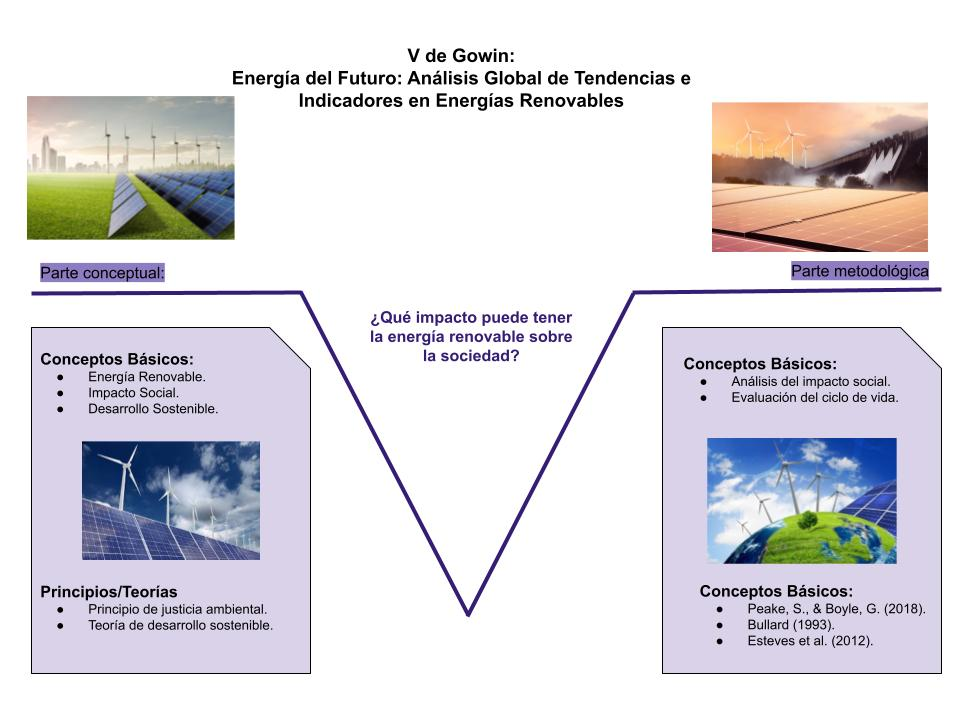
\includegraphics[width=1\textwidth,height=\textheight]{Dibujo-sin-título.jpg}

}

\caption{V de Gowin: Energía del Futuro}

\end{figure}%

\section{Parte de Escritura}\label{parte-de-escritura}

\textbf{Pregunta de investigación:} ¿Qué impacto puede tener la energía
renovable sobre la sociedad?

Para analizar los efectos que puede tener la energía renovable sobre la
sociedad, es importante entender no solo qué es la energía renovable,
sino también cómo ha sido estudiada y aplicada previamente. La energía
renovable se define como la energía derivada de recursos naturales que
se reponen continuamente, como la luz solar, el viento, el agua, la
biomasa y la energía geotérmica (United Nations, s.f.). Estas fuentes de
energía son abundantes y en todo el mundo se muestra la disponibilidad
de alguna de ellas, lo que las hace sumamente relevantes para la
transición hacia un futuro con energía más sostenible, y enfrentar los
inconvenientes del cambio climático.

En términos ambientales, la adopción de energías renovables puede
reducir considerablemente las emisiones de gases de efecto invernadero,
mejorando así la calidad del aire y disminuyendo los efectos negativos
del cambio climático en la salud pública (United Nations, s.f.). Esta
transformación, además de ser primordial para amortiguar los efectos
negativos del cambio climático, también es pertinente para lograr un
desarrollo sostenible.

Con el fin de responder la pregunta plenteada, se analizarán diversos
factores que inciden en la producción y utilización de energías
renovables. Entre estos destaca la disponibilidad de recursos naturales,
puesto que la eficiencia de la producción depende en gran medida de su
ubicación geográfica, las condiciones climáticas y los recursos
naturales presentes en la región (Casamitjana, 2017). Por ello, se
considerará además la inversión destinada a la investigación y el
desarrollo de nuevas tecnologías que permitan reducir las brechas entre
países.

Analizando desde una perspectiva económica, la energía renovable, aunque
en un inicio puede poner en riego el abastecimiento energético, debido a
la dificultad de esta transición, aunado además al costo elevado de la
inversión inicial (Casola y Freier, 2018); también tiene el potencial de
producir empleos e impulsar el desarrollo en comunidades locales. Según
``Energías Renovables'' (2011), el crecimiento de las industrias de
energía renovable puede generar millones de empleos nuevos en todo el
mundo, proporcionando oportunidades de trabajo en áreas rurales y
fomentando la independencia energética. Además, la implementación de
fuentes de energía renovable como la solar y la eólica puede reducir la
dependencia de los combustibles fósiles importados, fortaleciendo así la
seguridad energética de los países (Energías Renovables, 2011).

Si bien las energías renovables no garantizan por sí mismas un futuro
sostenible, es importante tomar en cuenta que las generaciones actuales
deben gestionar los recursos de manera eficiente, no solo para mejorar
su propio futuro, sino el futuro de las generaciones siguientes; pues de
no realizarse, el cambio climático seguirá acelerándose cada vez
más(Serrano, 2022). Así, la adopción de energías renovables puede
mejorar la calidad de vida, con un etorno menos contaminado que puede
traducirse en una mejor salud púlica y desarrollo económico.

Para detallar el problema de una forma clara, es importante señalar cómo
estas ventajas de la energía renovable pueden ser utilizadas para
descabezar las barreras presentes, como lo son los costos iniciales de
inversión y las limitaciones tecnológicas en algunas regiones. Este
enfásis ayuda que la pregunta escogida se contextualice dentro del marco
de desarrollo sostenible y transición energética que se requiere para
enfrentar los desafíos globales actuales.

Este enfoque pretende crear una estructura más clara que facilite
responder a la pregunta inicial, dando uso a información basada en las
fuentes citadas, y al mismo tiempo constituye una base sólida para el
desarrollo de una argumentación más especificada. Al emplear datos
relevantes y evidencia provenientes de organizaciones reconocidas, como
las Naciones Unidas y estudios especializados en energías renovables, se
garantiza que la discusión esté fundamentada en un conocimiento
actualizado y confiable. Además, integrar diferentes perspectivas, como
los beneficios ambientales, económicos y sociales, así como los desafíos
y las barreras para la implementación de energías renovables, ofrece una
punto de vista integral del problema que se espera estudiar. Esta
metodología no solo facilita la identificación de las áreas clave donde
se requiere cierto tipo de arbitraje, sino que también permite
considerar soluciones innovadoras y prácticas recomendadas que han sido
valiosas en otros contextos, enriqueciendo el análisis con ejemplos
concretos. El uso de una base de investigación sólida brinda un apoyo a
la construcción de un argumento persuasivo y bien fundamentado, que
puede guiar la toma de decisiones políticas y la implementación de
estrategias efectivas para promover la transición hacia un modelo
energético más sostenible.




\end{document}
